%
% Modelo LaTeX baseado no modelo A5L
% Adaptação para LaTeX por Bruno Ferreira

% Nota: usar /newpage com 1 coluna
%       usar /clearpage com 2 colunas
%       o /newpage com duas colunas escreve na próxima 
\documentclass[a5paper,twocolumn, 11pt]{article}
\usepackage[landscape]{geometry}

%Sample text
\usepackage{lipsum}

%escrever acentos e coisas do género sem que o latex se desoriente
\usepackage[utf8]{inputenc}

%hifenização e titulos em português
\usepackage[portuges]{babel}

%para ter a informação de quantas páginas tem o documento
\usepackage{lastpage}

%importar cores predefinidas
\usepackage[usenames,dvipsnames]{xcolor}
\definecolor{DarkGray}{gray}{0.40}

%usar multirow e multicolumn
\usepackage{multirow}

%para ter imagens, depois define a directoria de imagens
\usepackage{graphicx}
\graphicspath{{./imagens/}}

%definir o cabeçalho e rodapé
\usepackage{fancyhdr}
\pagestyle{fancy}
\fancyhead[L]{
    \small{
        \textcolor{DarkGray}{
            \textbf{Uminho 2012 - LI3 --- Transitários LEI}
        }
    }
}
\fancyhead[R]{
    \small{
        \textcolor{DarkGray}{
            \textbf{Pág. \thepage\ /\pageref{LastPage}}
        }
    }
}
\fancyfoot[C]{}

\begin{document}

\onecolumn
\thispagestyle{empty}
\begin{tabular}{ll}
    \multirow{7}{*}{ 
\includegraphics[height=90pt]{logo.jpeg} }
    &\\
    & \textcolor{DarkGray}{\Large{\textbf{Escola de Engenharia}}} \\
    &\\
    & \large{Departamento de Informática}\\
    &\\
    &\\
    & \large{Licenciatura em Engenharia Informática}\\
\end{tabular}
\begin{center}
    \Large{\textbf{Projecto de Laboratórios de Informática III}}\\
    \vspace{20pt}
    \Large{\textbf{``Transistários LEI --- Transporte de Carga''}}\\
    \vspace{15pt}
    \begin{tabular}{r@{, }l}
        Bruno Ferreira&A61055\\
        Daniel Carvalho&A61008\\
        Mariana Madeiros&A61041\\
    \end{tabular}
    
    \vspace{5pt}
    \emph{Grupo 42}\\\vspace{15pt}
    \large{\textbf{Braga, Março de 2012}}
\end{center}

\newpage
\tableofcontents

\newpage
\twocolumn
\section{Primeira secção}
\lipsum[1-2]
\begin{figure}[htb!]
    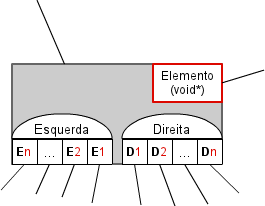
\includegraphics[width=190pt]{image2.png}
\end{figure}
\lipsum[1-3]

\clearpage
\section{Segunda secção}
\lipsum[1-1]
\begin{figure}[htb!]
    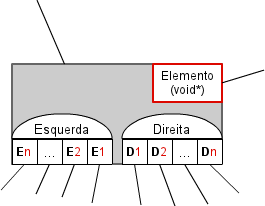
\includegraphics[width=190pt]{image2.png}
\end{figure}
\lipsum[1-1]

\newpage
\subsection{Uma subsecção}
\lipsum[1-3]

\clearpage
\onecolumn
\section{Fotos}
\begin{center}
    \begin{tabular}{ccc}
        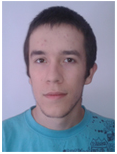
\includegraphics[width=90pt]{bruno.png}&
        
\includegraphics[width=90pt]{daniel.png}&
        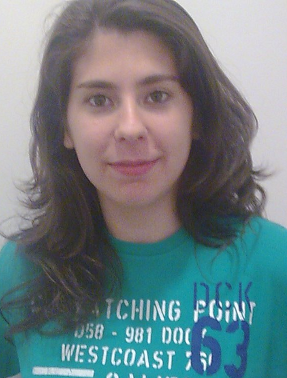
\includegraphics[width=90pt]{mariana.png}\\
        
        \small{\textbf{Bruno Ferreira}}&
        \small{\textbf{Daniel Carvalho}}&
        \small{\textbf{Mariana Medeiros}}\\
        \small{\textbf{A61055}}&
        \small{\textbf{A61008}}&
        \small{\textbf{A61041}}\\
    \end{tabular}
\end{center}
\end{document}